\documentclass[conference]{IEEEtran}
\IEEEoverridecommandlockouts

\usepackage{cite}
\usepackage{amsmath,amssymb,amsfonts}
\usepackage{algorithmic}
\usepackage{graphicx}
\usepackage{textcomp}
\usepackage{xcolor}
\usepackage{tikz}
\usepackage{float}

\def\BibTeX{{\rm B\kern-.05em{\sc i\kern-.025em b}\kern-.08em\kern-.1667em\lower.7ex\hbox{E}\kern-.125emX}}

\begin{document}

\title{Revisiting Rosenblatt Perceptron: Robust High-Entropy Classification via Uncertainty Margins}

\author{\IEEEauthorblockN{Anonymous Author(s) Affiliation omitted for double-blind review}}

\maketitle

\begin{abstract}
This paper addresses the challenge of deploying uncertainty-aware models in resource-constrained TinyML environments. While state-of-the-art architectures, such as LSTMs and Transformers, provide high representational capacity, their inference overhead and memory requirements are often prohibitive for edge applications. The present work develops a computationally efficient alternative: a modified linear perceptron featuring an adaptive selective prediction mechanism. 

By defining a geometric abstention region $[-\epsilon, \epsilon]$ around the decision hyperplane, the model implements a confidence-aware mechanism and selectively rejects low-confidence samples. Unlike static margin classifiers, the proposed $\epsilon$ parameter is derived from statistical properties estimated during training and calibration, while remaining fixed during inference, preserving a constant-time complexity of $\mathcal{O}(d)$.

The framework was evaluated across various high-entropy scenarios, including non-stationary financial time series, sentiment analysis (SemEval), and industrial fault detection (NASA IMS Bearing dataset). Experimental results demonstrate that the model achieves an inference memory footprint of $\approx 1$ KB and orders-of-magnitude lower computational overhead compared to recurrent neural networks. 

Furthermore, the selective mechanism enables the model to reach precision levels exceeding 90\% at reduced coverage of high-confidence predictions in industrial tasks. These findings suggest that robust feature engineering coupled with selective linear modeling provides a viable and energy-efficient path for reliable inference in hardware-limited settings.
\end{abstract}

\begin{IEEEkeywords}
Tiny Machine Learning, Simple Perceptron, Uncertainty Quantification, Selective Prediction, Feature Engineering, Time Series Forecasting, Non-stationary Data.
\end{IEEEkeywords}

\section{Introduction}

Modern machine learning models composed of multiple algebraic transformations (i.e. hidden layers) typically exhibit time complexity greater than $\mathcal{O}(n)$ per prediction, resulting in high computational costs during training, inference, and fine-tuning, particularly in edge embedded applications.

Such models identify patterns in raw data by applying geometrical transformations, processing the input layer by layer to extract increasingly abstract representations.

In contrast, feature learning can be replaced by feature engineering, where mathematical formulations are employed to encode relevant structures directly, rather than relying on hidden layers for representation learning. For instance, periodic structures can be efficiently captured using trigonometric functions such as sine and cosine functions to represent circular coordinates.

Following the introduction of the simple perceptron by Rosenblatt in 1957 \cite{b7}, Cover formalized the principle that \textit{“complex pattern classification problems, cast in a high-dimensional space nonlinearly...”} \cite{b2}. This observation suggests that nonlinear projections into higher-dimensional spaces increase the probability of achieving linear separability, enabling simple models to perform effectively in complex pattern recognition tasks.

\section{Background}

Linear models such as the simple perceptron \cite{b7} or linear regression \cite{b4} share the property of computing a linear combination of input features. In classification settings, this linear response is typically mapped to a binary window decision.

These models operate under the \textit{“formulation of the "general linear combination”} \cite{b4}. In the case of the simple perceptron, the model computes the dot product between the input feature vector and the corresponding vector, followed by the addition of bias term:

$$
z = \sum_{i=1}^{n} w_i x_i + b
$$

The resulting scalar value is then passed through an activation function. Each model employs a different activation depending on its objectives; for example, the simple perceptron uses a step function to produce binary output \cite{b7}.

$$
\hat{y} = f(z) = \begin{cases} 1 & \text{if } z \geq 0 \\ 0 & \text{if } z < 0 \end{cases}
$$

However, while individual linear units (weights) are computationally efficient, modern Deep Neural Networks stack multiple layers of these operations, resulting in millions of parameters. This scale presents a challenge for deployment on embedded systems with limited memory.

In the mid-20th century, something similar to a \textit{“machine learning winter”} occurred. Models such as the simple perceptron lacked the geometric capacity to solve problems such as XOR \cite{b6}, leading to the dropout of these models and their use was only retained as a foundation for subsequent generations of models.

Although the non-linear limitations of the simple perceptron with respect to the XOR problem led to the prioritization of multi-layer architectures \cite{b6}, current energy constraints in edge computing warrant a re-evaluation of linear models when coupled with robust feature engineering.

\section{Related Work}

"A diverse set of techniques has been developed to quantify model uncertainty. Bayesian Neural Networks (BNNs) leverage probabilistic parameters to localize low-confidence regions. However, BNNs typically rely on Monte Carlo sampling during inference, which is computationally prohibitive for micro-controller-based TinyML. Similarly, Support Vector Machines (SVMs) optimize a static separation margin with $\mathcal{O}(n^2)$ training complexity, limiting their adaptability to non-stationary data streams.

Other model families, such as ProtoNN and Bonsai \cite{b11}, are tailored for embedded or otherwise resource-limited settings, offering low computational complexity while preserving competitive accuracy. These approaches are often employed in safety-critical domains (e.g., fault diagnosis in engineered systems), where incorrect decisions may lead to serious consequences. To reduce such risks, the proposed uncertainty-aware perceptron follows a similar philosophy, using data dispersion as the basis for quantifying predictive confidence.

Unlike SVMs, which determine a fixed separating margin through a computationally demanding training process with complexity on the order of $\mathcal{O}(n^2)$, the geometric margin $\epsilon$ in the proposed approach is computed from statistical descriptors (e.g., the empirical standard deviation $\sigma$) learned during training and calibration. This design maintains an inference complexity of $\mathcal{O}(d)$, where $d$ is the dimensionality of the input.

Current machine learning research often prioritizes representation learning architectures (e.g., LSTMs or Transformers). However, for non-stationary time-series, the computational burden of learning temporal dependencies can in many cases be replaced by trigonometric cyclic encoding and stochastic oscillators \cite{b12}. Shifting from “learning the structure” to explicitly “encoding the structure” allows linear models to remain competitive in high-entropy settings, especially when selective prediction and reliability-oriented performance metrics are used.

\section{Linear Decision Hyperplane with Marginal Uncertainty}

To quantify uncertainty ($\epsilon$) in the simple perceptron, the geometry of the step function defines the region in which the weighted sum lies for positive (1) and negative (0) predictions.

The modified decision function is defined as:

\[
h(z) =
\begin{cases}
1   & \text{if } z > \epsilon \\
0   & \text{if } z < -\epsilon \\
0.5 & \text{if } -\epsilon \leq z \leq \epsilon
\end{cases}
\]

The introduction of the region $[-\epsilon, \epsilon]$ transforms the usual decision into a geometric margin. Following the principles established by Cortes and Vapnik, maximizing the distance of data points from the separating hyperplane improves generalization \cite{b9}. This approach is consistent with modern selective classification strategies that prioritize precision over coverage \cite{b13}.

\begin{figure}[H]
    \centering
    \caption{Uncertainty Step Function}
    \label{tab:Uncertainty-Step-Function}
    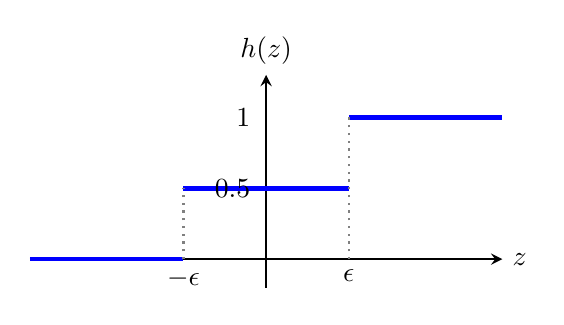
\begin{tikzpicture}[x=1.5cm, y=1.8cm, thick, >=stealth]
        \draw[->] (-2,0) -- (2,0) node[right] {$z$};
        \draw[->] (0,-0.2) -- (0,1.3) node[above] {$h(z)$};
    
        \def\ep{0.7}
    
        \draw[blue, ultra thick] (-2,0) -- (-\ep,0) (-\ep,0.5) -- (\ep,0.5) (\ep,1) -- (2,1);
    
        \draw[gray, dotted] (-\ep,0) node[below, black]{$-\epsilon$} -- (-\ep,0.5);
        \draw[gray, dotted] (\ep,0)  node[below, black]{$\epsilon$}  -- (\ep,1);
    
        \node[left, xshift=-2pt] at (0,0.5) {$0.5$};
        \node[left, xshift=-2pt] at (0,1) {$1$};
    \end{tikzpicture}
\end{figure}

Unlike static margins in SVMs, the proposed $\epsilon$ introduces an uncertainty-aware margin, forcing the perceptron to continue updating its weights when samples fall within the uncertainty region ($h(x) = 0.5$), indicating insufficient geometric distance from the decision boundary.

The uncertainty parameter ($\epsilon$) is a constant defined prior to each prediction, introducing a gray region around the "decision border". The model outputs a positive prediction (1) when the linear activation ($z$) exceeds the uncertainty threshold ($\epsilon$). 

When $z$ is below the negative region, the prediction is negative (0). If neither condition is satisfied, the prediction falls in the uncertainty region, yielding an indeterminate or outlier case (0.5).

To compute the uncertainty margin of the model, the standard deviation ($\sigma$) is proposed, which Karl Pearson defined as \textit{"...a natural measure of the "scatter" of observations."} \cite{b10}. 

In high-dimensional spaces, the standard deviation ($\sigma$) indicates the level of dispersion and noise in the data; this standard deviation must be calculated for each of the training data in the hyperplane of the model, where the uncertainty margin $\sigma$ is estimated during training and calibration and remains fixed during inference.

$$
\sigma = \sqrt{\frac{1}{N} \sum_{i=1}^{N} (x_i - \mu)^2}
$$

The proposed formula to compute model uncertainty begins by defining an external margin to calibrate the model sensitivity ($\Delta$), obtained by multiplying the ratio of the standard deviation ($\sigma$) to the error rate—scaled between 0 and 1 ($\text{E}$). 

This function, based on a Gaussian formulation, adjusts the confidence of the model as a function of the observed error rate ($\text{E} = (\text{Number of Errors in Training} / \text{Total Attempts}) * 100\%$) when the error rate is low, the predictions of the model become more reliable; conversely, higher error rates indicate a reduced confidence.

$$
\epsilon = \Delta \cdot \sigma \cdot Z_{(1 - \frac{E}{2})}
$$

\section{Model Learning Rule}

During each learning epoch, the model updates its parameters using the Perceptron learning rule \cite{b7}. The weight adjustment is calculated as the product of the learning rate ($\eta$) and the prediction error, defined as the difference between the true label ($y$) and the predicted output of the perceptron ($\hat{y}$), which is obtained from the activation step function (0 or 1).

The weight update rule ($w$) is defined as:

$$
w_i \leftarrow \eta (y - \hat{y}) x_i
$$

Similarly, the bias ($b$) is updated as follows:

$$
b \leftarrow b + \eta (y - \hat{y})
$$

\section{Model Vectorization and Feature Representation}

In order to construct an algebraic representation for linear modeling, the raw time-series data are transformed into a structured  input vector using a set of operations.

The objective of this vectorization process is to represent diverse temporal, statistical, and dynamical properties of the signal in a high-dimensional space, increasing the probability of achieving linear separability.

The resulting input vector ($v$) is composed of three characteristic groups: indicators that capture the structure of the time-series, cyclic time encoding to preserve the periodic structure, and normalized statistical attributes to ensure the appropriate data scale.

\subsection{Non-Stationary Indicator Features}

Here, the raw data vector is $x$. A set of indicators are used as statistical metrics to represent the time-performance and health of the data.

The results presented in this work are obtained using a specific set of indicators, which introduces non-linear transformations of the original raw values, expanding the representational capacity of the linear model.

For the vector $x$, each element is denoted by $x_i$; the maximum and minimum values are given by $x_{\max}$ and $x_{\min}$, and the last element is denoted by $x_n$.

The stochastic oscillator is defined as:

$$
\%K = \frac{x_n - x_{\min}}{x_{\max} - x_{\min}} \cdot 100
$$

Given the vector $x$, the positive and negative gradients are computed as a separate list. The gain vector $G$ is defined such that $G_i$ contains positive changes and zero otherwise. In contrast, the negative gradient vector $L$ contains the absolute value of negative changes and zero otherwise.

Relative strength (RS) is computed as:

$$
RS = \frac{\frac{1}{n} \sum_{i=1}^{n}G_i}{\frac{1}{n} \sum_{i=1}^{n}L_i}
$$

From which the Relative Strength Index (RSI) is derived:

$$
RSI = 100 - \frac{100}{1 + RS}
$$

To capture temporal smoothing and exponential decay, the Exponential Moving Average (EMA) is computed as:

$$
EMA_{\text{initial}} = SMA = \frac{\sum_{i=1}^{n}x_i}{n}
$$

$$
EMA_t = EMA_{t-1} + \alpha(x_n - EMA_{t-1})
$$

with smoothing factor:

$$
\alpha = \frac{2}{n + 1}
$$

In the representation of cyclic time encoding, these models learn to develop a sense of time (e.g., month, week, hour, etc.). The model uses these functions to represent the "coordinates" in the selected timestamp.

$$
v = \frac{2\pi \cdot t}{T}
$$

$$
\sin(v), \quad \cos(v)
$$

The Z-score normalization is implemented to scale the external values using a consistent scale (computed across the training data set partition), where $\sigma$ represents the standard deviation of $x$.

$$
z = \frac{x_n - (\frac{1}{n} \sum_{i=1}^{n} x_i)}{\sigma}
$$

Although a significant amount of work is done through feature engineering, the proposed model remains the one that is capable of filtering noise, finding a high-dimensional hyperplane, and identifying a “noise” pattern within the data. All of which are achieved through the model’s fine-tuning capabilities.

\section{Non-stationary Dataset and Data Preprocessing}

\subsection{Non-stationary Selected Dataset}

During training, various high-noise and non-stationary datasets were used for model testing. To validate the model in environments where large amounts of data are easily available, several historical corporate data were selected.

These datasets were chosen because historical corporate environments allow the model to be subjected to extreme noise stress over long periods (up to the last 10 years).

\subsection{Dataset Management}

To ensure proper data collection and avoid data leakage, the entire data set was divided into separate subsets for training and post-training testing.

A sliding-window algorithm (using a window length of 14) was implemented to iterate over the current and past data window. The model was explicitly prevented from accessing future data.

\subsection{Approach}

With the split data set, the model was trained as usual, following the Rosenblatt approach \cite{b7}. After completion of the full training phase, uncertainty was added during post-training testing, and the model was run across the entire dataset using the same sliding-window approach.

\subsection{Non-stationary Data Results}

Hereafter, the section presents all the results obtained from experiments conducted across various distinct high-noise environments, together with the computational resources employed and the corresponding approximate execution times, including: data post-processing, training, and inference.

\begin{table}[H]
    \centering
    \caption{Dataset Signal Profiles \& Characteristics}
    \label{tab:Timestamp-Window-Sequential-Set}
    \begin{tabular}{c c c}
        \hline
        Dataset ID & Volatility Profile ($\sigma$) & Duration (yrs)\\
        \hline
        Type I & $\sigma \approx 0.58$ & 2.75\\
        Type II & $\sigma \approx 0.31$ & 9.5\\
        Type III & $\sigma \approx 0.23$ & 7.3\\
        Type IV & $\sigma \approx 0.26$ & 2.9\\
        \hline
        \multicolumn{3}{p{0.9\linewidth}}{\centering
        Sampled at 15-minute time steps. $\sigma$ represents the annualized standard deviation of the dataset, for the noisy density. Type I: TSLA, Type II: GOOGL, Type III: Eli Lilly, Type IV: APPL.
        }
    \end{tabular}
\end{table}

\begin{table}[H]
    \centering
    \caption{Training Time}
    \label{tab:Training-Time-Sequential-Set}
    \begin{tabular}{c c c}
        \hline
        Dataset Type & Time (seconds) & Training Vectors\\
        \hline
        Type I & $\approx3.34$ sec & $\approx40000$\\
        Type II & $\approx9.44$ sec & $\approx110000$\\
        Type III & $\approx6.14$ sec & $\approx80000$\\
        Type IV & $\approx3.74$ sec & $\approx37000$\\
        \hline
        \multicolumn{3}{p{0.9\linewidth}}{\centering
        Obtained results include processing and prepossessing time, during the training.
        }
    \end{tabular}
\end{table}

\begin{table}[H]
    \centering
    \caption{Total Training Accuracy (in all the dataset, without uncertainty)}
    \label{tab:Total-Accuracy-Sequential-Set}
    \begin{tabular}{c c}
        \hline
        Dataset Type & Total Accuracy\\
        \hline
        Type I & $\approx56.1\%$\\
        Type II & $\approx55.31\%$\\
        Type III & $\approx56.34\%$\\
        Type IV & $\approx56.84\%$\\
        \hline
        \multicolumn{2}{p{0.9\linewidth}}{\centering
        Dataset was split into approximately $\approx\%73$ for training, corresponding to approximately $\approx\%27$ for testing.
        }
    \end{tabular}
\end{table}

\begin{table}[H]
    \centering
    \caption{Uncertainty Accuracy (proportion of coverage:accuracy)}
    \label{tab:Uncertainty-Accuracy}
    \begin{tabular}{c c c}
        \hline
        Dataset Type & Small Coverage & Medium Coverage\\
        \hline
        Type I & $\approx17\%:\approx97\%$ & $\approx47\%:\approx68\%$\\
        Type II & $\approx23\%:\approx93\%$ & $\approx43\%:\approx67\%$\\
        Type III & $\approx21\%:\approx89\%$ & $\approx52\%:\approx68\%$\\
        Type IV & $\approx23\%:\approx93\%$ & $\approx42\%:\approx69\%$\\
        \hline
        \multicolumn{3}{p{0.9\linewidth}}{\centering
        The section presents the coverage and accuracy obtained on that data partition after incorporating the uncertainty function, using different sensibilities.
        }
    \end{tabular}
\end{table}

\section{Sentiment Analysis Dataset and Data Preprocessing}

To demonstrate that this model not only works with long non-stationary data, it was also challenged against a dataset for sentiment analysis, classified as positive (1) or negative (0). The data set selected for this task was SemEval, a data set that labels data from a social network as positive or negative, thereby demonstrating the convergence of this model when applied to natural language processing tasks.

For data preparation, N-grams were used and a corresponding scale was created to normalize the characters between 0 and 1. Finally, for data analysis, techniques similar to those used in convolutional neural networks were applied, where the model operates in a manner similar to a sliding window over the sequence, performing inference depending on the size of the respective input vector.

\subsection{Sentiment Data Results}

\begin{table}[H]
    \centering
    \caption{Natural Language Processing Results}
    \label{tab:NLP-SemEval}
    \begin{tabular}{c c c}
        \hline
        Category & Accuracy & Other\\
        \hline
        Total Coverage & $\approx69.4\%$ & N/A\\
        Selected Coverage & $93.7\%$ & $\approx79.3\%$ Coverage\\
        Model Dimensions & 1080 & N/A\\
        Training Time & $\approx9$ sec & N/A\\
        \hline
        \multicolumn{3}{p{0.9\linewidth}}{\centering
        The section presents the total coverage, selected, model dimensions (in this case, the dimensionality corresponds to the number of n-grams or bag-of-words features) and training time.
        }
    \end{tabular}
\end{table}

\section{Industrial Validation: NASA Bearing Dataset}

To further validate the model in a critical embedded sensing scenario, the NASA IMS Bearing Dataset has been utilized. This task involves a binary classification of the bearing state (Healthy:1 vs. Faulty:0) based on vibration accelerometer data.

Unlike the stochastic nature of markets, mechanical degradation follows physical laws, yet early fault detection remains challenging due to signal noise in transition states. For this task, a low-dimensional input vector has been engineered, consisting of Root Mean Square (RMS), harmonic oscillators, sin, cos, Kurtosis, Crest Factor, and Skewness, computed over sliding windows.

\subsection{Industrial Data Results}

The proposed model demonstrated exceptional efficiency in this domain, effectively filtering out transition noise to provide reliable early warnings.

\begin{table}[H]
    \centering
    \caption{Performance on NASA Bearing Dataset}
    \label{tab:NASA-Results}
    \begin{tabular}{c c c}
        \hline
        Category & Accuracy & Other\\
        \hline
        Total Coverage & $\approx79.4\%$ & N/A\\
        Selected Coverage & $94.7\%$ & $\approx40\%$ Coverage\\
        Model Dimensions & 14 & N/A\\
        Training Time & $\approx6.4$ sec & N/A\\
        \hline
        \multicolumn{3}{p{0.9\linewidth}}{\centering
        By rejecting uncertain samples during the transient degradation phase, the model achieves near-perfect accuracy in confirmed states, acting as a robust low-power early warning system.
        }
    \end{tabular}
\end{table}

\section{Used Hardware}

The hardware used during training consisted of a single 64-bit CPU core and approximately $\approx 1$ MB of RAM. During the inference phase, the model used only $\approx 1$ KB of memory, since it did not need to load the data set into memory.

Similarly, the model was tested on a t2.micro server within the AWS architecture. Running on this hardware, the same resource usage metrics were observed.

\section{Mathematical Analysis}

The primary distinction of the proposed model lies in its reduced time complexity and minimal memory footprint. Before formal analysis, this section elucidates the underlying mathematical foundations and the specific calculations for each component of the model.

\begin{table}[H]
    \centering
    \caption{Time Complexity and Memory Space}
    \label{tab:Mathematical-Analysis}
    \begin{tabular}{c c c}
        \hline
        Stage & Time Complexity & Memory Space\\
        \hline
        Training & $\mathcal{O}(e * n * d)$ & $\mathcal{O}(d)$\\
        Inference & $\mathcal{O}(d)$ & $\mathcal{O}(d)$\\
        Input Vector & $\mathcal{O}(d * l)$ & $\mathcal{O}(d)$\\
        Uncertainty Function & $\mathcal{O}(1)$ & $\mathcal{O}(1)$\\
        \hline
        \multicolumn{3}{p{0.9\linewidth}}{\centering
        e = epochs, n = samples, d = features, l = length
        }
    \end{tabular}
\end{table}

\section{Comparison}

Following the methodological framework of this document, a comparative analysis is presented against various machine learning architectures. This evaluation rigorously focuses on time complexity ($\mathcal{O}$), spatial resource allocation (memory footprint), and operational capabilities within high-entropy environments.

The selected models for this comparison—Bonsai \cite{b11}, FastGRNN \cite{b12}, and ProtoNN \cite{b11}—were chosen based on their established performance in TinyML benchmarks.

\begin{table}[H]
    \centering
    \caption{Time Complexity}
    \label{tab:Time-Complexity-Comparation}
    \begin{tabular}{c c c}
        \hline
        Model & Training & Inference\\
        \hline
        Proposed & $\mathcal{O}(e * n * d)$ & $\mathcal{O}(d)$\\
        Bonsai & $\mathcal{O}(e * n * d  * depth)$ & $\mathcal{O}(d * depth)$\\
        FastGRNN & $\mathcal{O}(e * n * d * l)$ & $\mathcal{O}(d * l)$\\
        ProtoNN & $\mathcal{O}(e * n * d * k)$ & $\mathcal{O}(d * k)$\\
        Linear SVM & $\mathcal{O}(n^2 * d)$ & $\mathcal{O}(d)$\\
        Standard LSTM & $\mathcal{O}(e * n * l * d^2)$ & $\mathcal{O}(l * d^2)$\\
        \hline
    \end{tabular}
\end{table}

\begin{table}[H]
    \centering
    \caption{Estimated Hardware Usage}
    \label{tab:Estimated-Hardware-Usage-Comparation}
    \begin{tabular}{c c c}
        \hline
        Model & Space in Memory (RAM) & Latency\\
        \hline
        Proposed & $\approx1$ KB & $\approx9$ ms\\
        Bonsai & $\approx4.5$ KB & $\approx13$ ms\\
        FastGRNN & $\approx47$ KB & $\approx12$ ms\\
        ProtoNN & $\approx16$ KB & $\approx13$ ms\\
        Linear SVM & $\approx2$ KB & $\approx10$ ms\\
        Standard LSTM & $>500$ KB & $\approx13$ sec\\
        \hline
        \multicolumn{3}{p{0.9\linewidth}}{\centering
        Benchmarks were conducted on a constrained virtualized environment (single-core 64-bit CPU, 1 MB RAM limit) to simulate resource scarcity in embedded systems. The reported latency included the time required for feature preprocessing.
        }
    \end{tabular}
\end{table}

\begin{table}[H]
    \centering
        \caption{Natural Language Tasks (SemEval Dataset)}
    \label{tab:NLP-SemEval-Comparation}
    \begin{tabular}{c c c}
        \hline
        Model & Total Accuracy & Selected:Accuracy\\
        \hline
        Proposed & $\approx69.4\%$ & $\approx79.3\%:\approx93.7\%$\\
        Bonsai & $\approx69.8\%$ & N/A\\
        FastGRNN & $\approx70.8\%$ & N/A\\
        ProtoNN & $\approx68.4\%$ & N/A\\
        Linear SVM & $\approx67.2\%$ & N/A\\
        Standard LSTM & $\approx70.1\%$ & N/A\\
        \hline
    \end{tabular}
\end{table}

\section{Implications and Future Work}

Current ongoing research is focused on extending this uncertainty mechanism from a passive filter to an active learning trigger, a framework tentatively titled \textit{Epsilon Recurrent Feedback for Linear Models}.

Although current work uses $\epsilon$ to abstain from prediction, future iterations aim to utilize the uncertainty region as a routing signal to bridge the gap between linear and deep representations. The proposed framework envisions a hierarchical architecture in which uncertainty-driven routing enables adaptive model escalation.

\begin{itemize}

    \item Selective Escalation: Input vectors falling within the uncertainty margin ($\epsilon$) are not discarded but are instead escalated to a High-Capacity Model (e.g., a Transformer or Large Language Model) acting as a teacher.
    
    \item Closed-Loop Distillation: The high-confidence labels generated by the oracle for these "hard" samples are fed back into the linear model. This creates a continuous knowledge distillation cycle, allowing the simple perceptron to asymptotically approximate the decision boundaries of deeper architectures while maintaining $\mathcal{O}(1)$ inference costs for the majority of traffic.
    
    \item Contextual Adaptation: Future work will also explore the integration of context-aware weights using Exponential Moving Averages (EMA) to handle temporal dependencies without the overhead of Recurrent Neural Networks (RNNs).
    
\end{itemize}

Preliminary experiments with this feedback loop in OWASP datasets suggest that it is possible to compress the knowledge of large-scale models into linear weights, effectively solving the "Linear vs. Deep" trade-off for resource-constrained environments.

\section{Conclusion}

This work presents an uncertainty-aware linear perceptron designed for extreme edge constraints. The model demonstrates a training complexity of $\mathcal{O}(e * n * d)$ and a constant inference cost of $\mathcal{O}(d)$, using approximately 1 KB of memory. Furthermore, feature preprocessing remains efficient with an average complexity of $\mathcal{O}(n)$, allowing operation within 100-byte buffers. The results illustrate Cover's theorem in practice, effectively filtering noise in high-entropy environments. 

Crucially, this shows that the model's objective is not universal coverage but rather achieving high precision ($>90\%$) through selective coverage. This approach offers orders-of-magnitude reductions in computational costs compared to RNNs, proving that robust feature engineering coupled with selective linearity is a viable path for reliable TinyML.

\section{Acknowledgment}

Acknowledgments omitted for double-blind review.

\section{Resources}

GitHub repository omitted for double-blind review.

\begin{thebibliography}{00}
\bibitem{b1} K. Cho et al., "Learning phrase representations using RNN encoder-decoder for statistical machine translation", 2014.
\bibitem{b2} T. M. Cover, "Geometrical and statistical properties of systems of linear inequalities with applications in pattern recognition", 1965.
\bibitem{b3} S. Hochreiter and J. Schmidhuber, "Long Short-Term Memory", 1997.
\bibitem{b4} A. M. Legendre, "Nouvelles méthodes pour la détermination des orbites des comètes. Courcier", 1805.
\bibitem{b5} F. T. Liu, K. M. Ting, and Z. H. Zhou, "Isolation forest", 2008.
\bibitem{b6} M. Minsky and S. Papert, "Perceptrons: An Introduction to Computational Geometry", 1969.
\bibitem{b7} F. Rosenblatt, "The perceptron: A probabilistic model for information storage and organization in the brain", 1958.
\bibitem{b8} S. Tuli, G. Casale, and N. R. Jennings, "TranAD: Deep transformer networks for anomaly detection in multivariate time series", 2022.
\bibitem{b9} C. Cortes and V. Vapnik, "Support-vector networks", Machine Learning, 1995.
\bibitem{b10} K. Pearson, "Contributions to the Mathematical Theory of Evolution", 1894.
\bibitem{b11} A. Kumar, S. Goyal, and M. Varma, "Resource-efficient Machine Learning in 2 KB RAM for the Internet of Things", ICML, 2017.
\bibitem{b12} A. Kusupati et al., "FastGRNN: A Fast, Accurate, Stable and Tiny RNN for Edge Computing", NeurIPS, 2018.
\bibitem{b13} Y. Geifman and R. El-Yaniv, "Selective classification for deep neural networks", NeurIPS, 2017.
\end{thebibliography}

\end{document}